\chapter{Diseño\label{cap:disenho}}

TODO: [Introducción]


\section{Arquitectura\label{sec:dis:arquitectura}}

TODO: Arquitectura
  {Front-End/Back-End}
  Ventajas de la división en front-end/back-end
  Esquema comunicación front-end/back-end
  Red interna, necesidad

\section{Back-End - Servicio Web FPGA\label{sec:dis:servicio_web_fpga}}

TODO: 
  {REST-like,asíncrono}
  Peticiones rest, cluster, arquitectura

\begin{figure}[!htp]
  \centering
  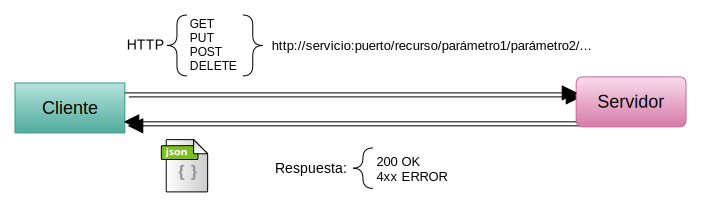
\includegraphics[width=\textwidth,clip=true]{fpga_rest}
  \caption{Diagrama de flujo de un servicio \gls{REST}.}
  \label{fig:fpga_rest}
\end{figure}

\begin{figure}[!htp]
  \centering
  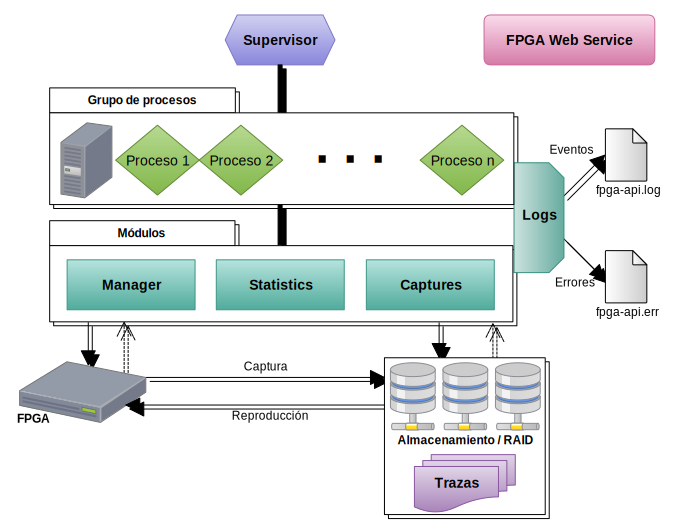
\includegraphics[width=\textwidth,clip=true]{fpga}
  \caption{Máquina de Estados Finita para el estado de la \gls{FPGA}.}
  \label{fig:arquitectura_servicio}
\end{figure}

\begin{figure}[!htp]
  \centering
  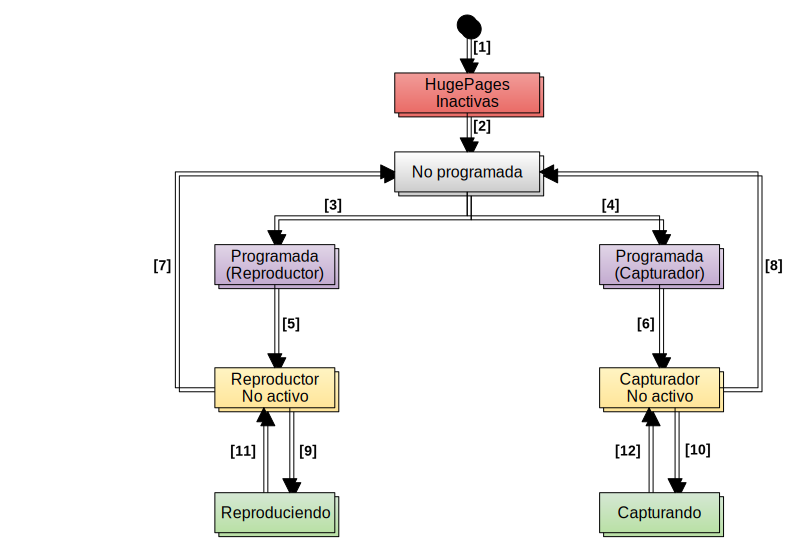
\includegraphics[width=\textwidth,clip=true]{fpga_estado}
  \caption{Arquitectura del \gls{servicioweb} \gls{FPGA}.}
  \label{fig:fpga_estado}
\end{figure}

Submódulos be like:

\subsection{Gestión\label{ssec:dis:gestion}}

TODO: Gestión
  {Capturador,Reproductor}


\subsection{Capturas\label{ssec:dis:capturas}}

TODO: Capturas
  {Detección,Conversión,Renombrado,Borrado}


\subsection{Estado/Estadísticas\label{ssec:dis:estado_estadisticas}}

TODO: Estado/Estadísticas
  {Velocidad,Estado,RAID}


\section{Front-End - Interfaz web\label{sec:dis:interfaz_web}}

TODO: [Introducción]

TODO: Interfaz Gráfica, utilización del framework
  {Diseño responsive,localización}
  {Maquetas}
  Páginas - maquetas

\subsection{Maquetas\label{ssec:dis:maquetas}}

\begin{figure}[!htp]
  \centering
  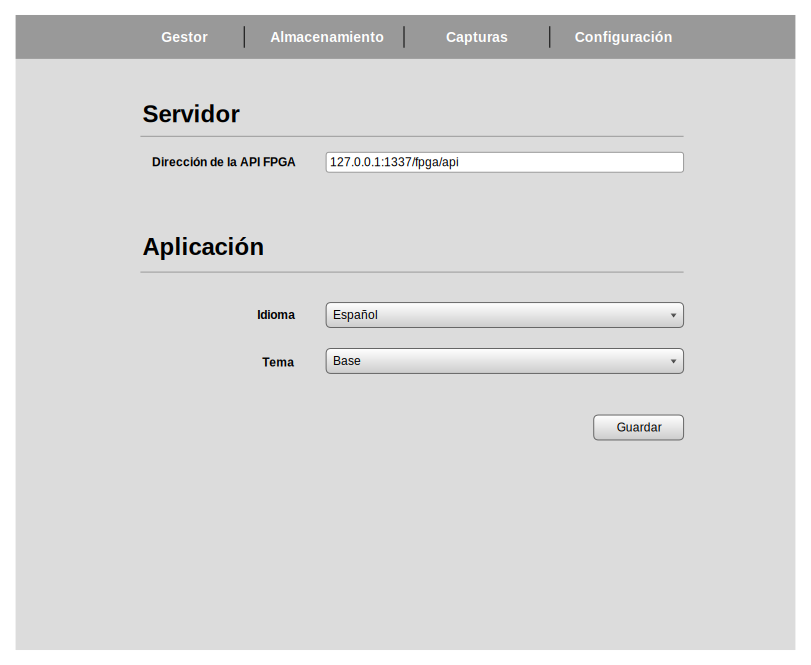
\includegraphics[width=\textwidth,clip=true]{maquetas/maqueta_configuracion}
  \caption{Maqueta de la pantalla de configuración de la aplicación.}
  \label{fig:maqueta:configuracion}
\end{figure}

\begin{figure}[!htp]
  \centering
  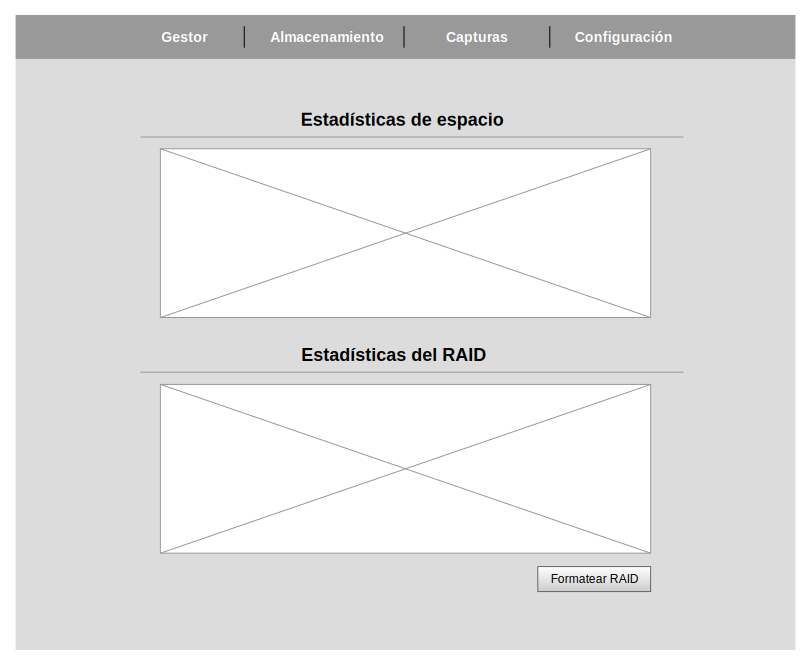
\includegraphics[width=\textwidth,clip=true]{maquetas/maqueta_almacenamiento}
  \caption{Maqueta de la pantalla de almacenamiento.}
  \label{fig:maqueta:almacenamiento}
\end{figure}

\begin{figure}[!htp]
  \centering
  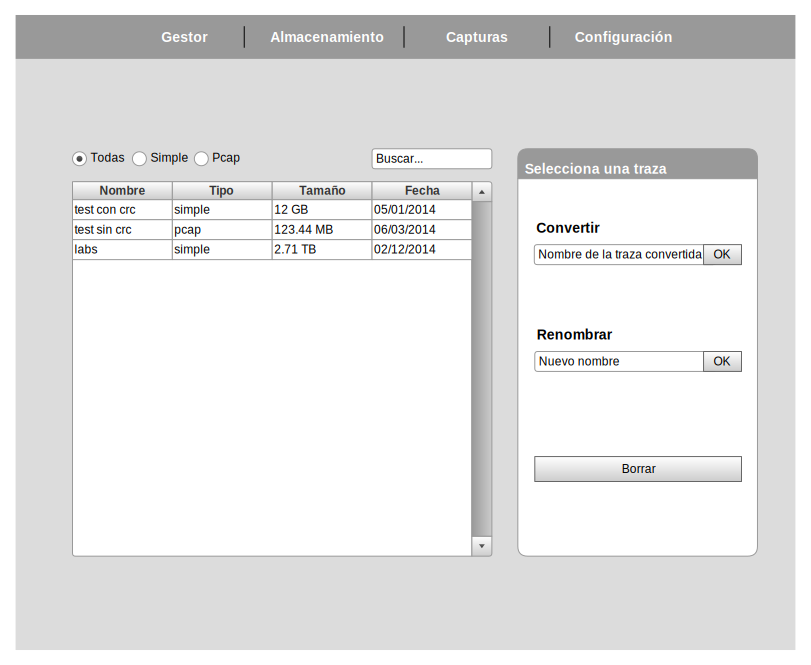
\includegraphics[width=\textwidth,clip=true]{maquetas/maqueta_capturas}
  \caption{Maqueta de la pantalla de gestión de \glspl{traza}.}
  \label{fig:maqueta:capturas}
\end{figure}

\begin{figure}[!htp]
  \centering
  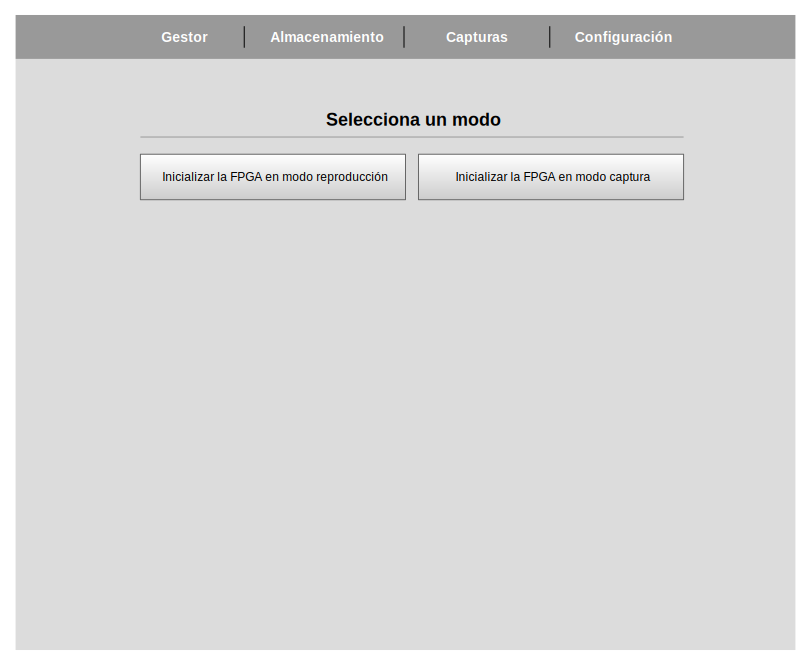
\includegraphics[width=\textwidth,clip=true]{maquetas/maqueta_gestor_seleccion}
  \caption{Maqueta de la pantalla de gestión - selección de modo.}
  \label{fig:maqueta:gestor_seleccion}
\end{figure}

\begin{figure}[!htp]
  \centering
  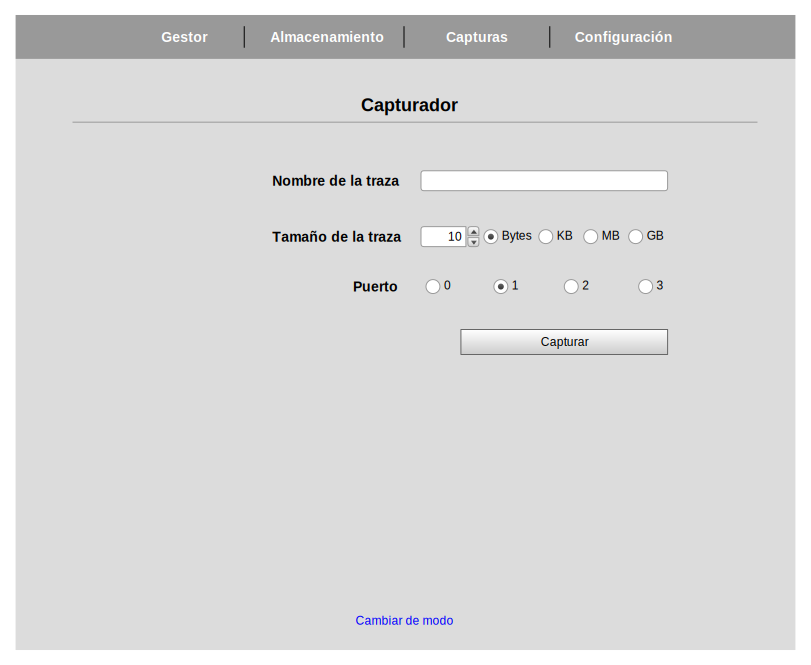
\includegraphics[width=\textwidth,clip=true]{maquetas/maqueta_gestor_capturador}
  \caption{Maqueta de la pantalla de gestión - formulario para capturar.}
  \label{fig:maqueta:gestor_capturador}
\end{figure}

\begin{figure}[!htp]
  \centering
  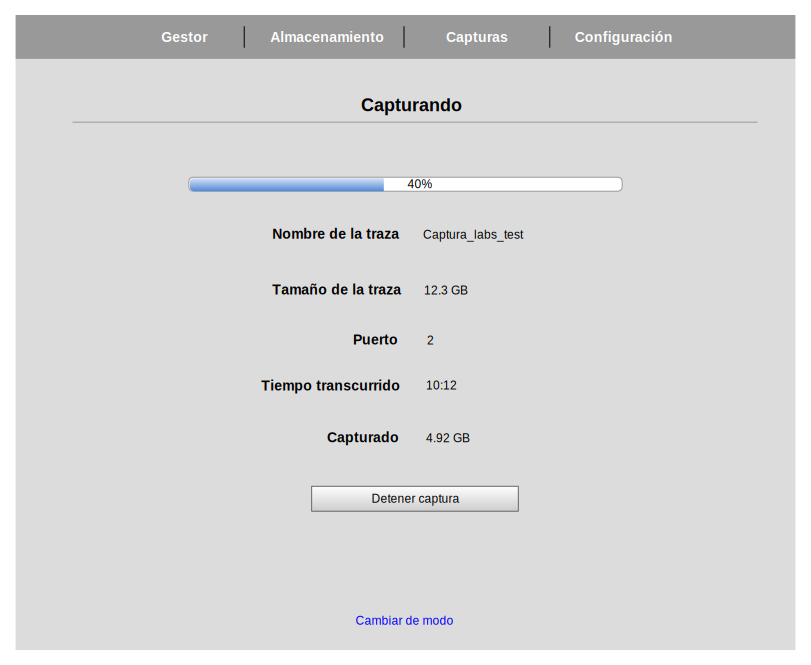
\includegraphics[width=\textwidth,clip=true]{maquetas/maqueta_gestor_capturando}
  \caption{Maqueta de la pantalla de gestión - capturando.}
  \label{fig:maqueta:gestor_capturando}
\end{figure}

\begin{figure}[!htp]
  \centering
  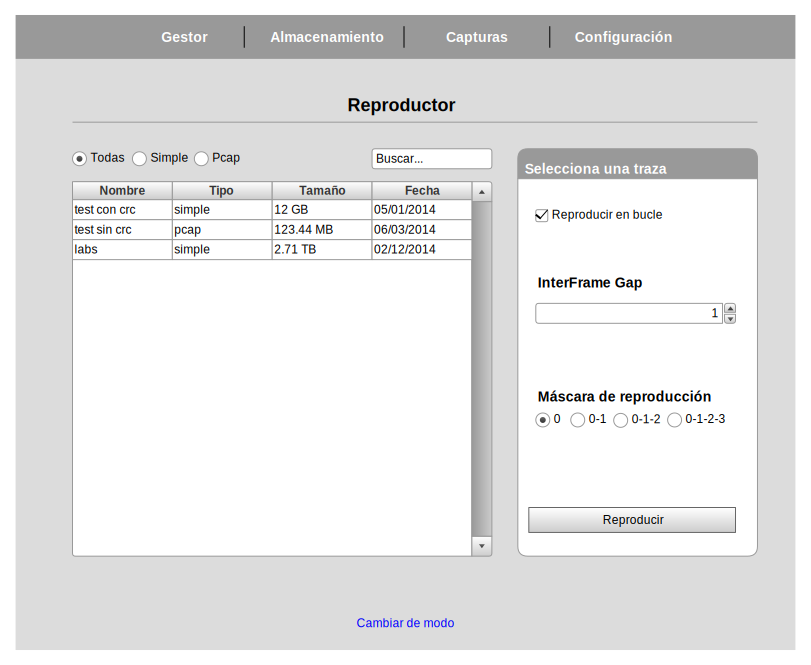
\includegraphics[width=\textwidth,clip=true]{maquetas/maqueta_gestor_reproductor}
  \caption{Maqueta de la pantalla de gestión - formulario para reproducir.}
  \label{fig:maqueta:gestor_reproductor}
\end{figure}

\begin{figure}[!htp]
  \centering
  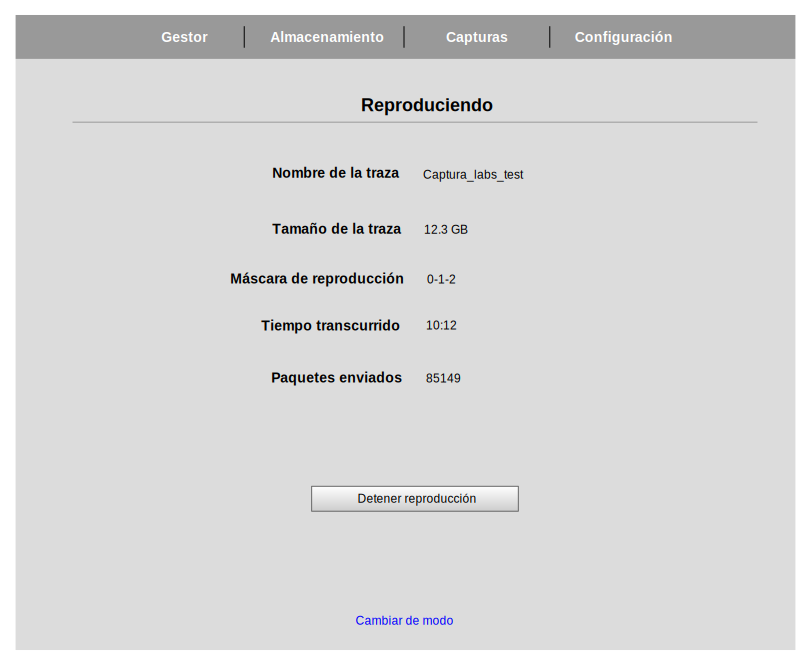
\includegraphics[width=\textwidth,clip=true]{maquetas/maqueta_gestor_reproduciendo}
  \caption{Maqueta de la pantalla de gestión - reproduciendo.}
  \label{fig:maqueta:gestor_reproduciendo}
\end{figure}